\chapter{Literature Survey}
\label{chapter:literature-survey}

Following on from the introduction, \Cref{chapter:literature-survey} comprehensively reviews the existing knowledge pertinent to this research by building a ``Problem-Gap-Solution" narrative. First, we introduce the \textbf{Problem}, covering the challenges of the global seafood industry such as mislabeling and adulteration. The chapter then discusses the technological \textbf{Landscape}, reviewing existing analytical techniques for seafood authentication with a focus on Rapid Evaporative Ionization Mass Spectrometry (REIMS). Next, we establish the \textbf{Gap} by presenting a focused literature review on the state of REIMS data analysis, tracing its evolution from foundational PCA/LDA, through chemometric OPLS-DA, to the most recent applications of foundational machine learning and ANNs. This review identifies the limitations of current methods and establishes the need for more advanced models. Subsequently, the chapter details the \textbf{Solution}, introducing the suite of advanced deep learning architectures that form the core of this thesis, including Transformers, Mixture of Experts, and strategies like Transfer Learning and Contrastive Learning. Finally, we address the critical component of \textbf{Validation} by discussing Explainable AI as a tool for building trust in these complex models.

\section{The Challenges of Seafood Integrity: Fish Processing, Fraud, and Contamination}

The global fish processing industry is a critical part of our food supply chain; it transforms marine biomass (i.e., a collective term for every single living organism in the ocean) into a wide variety of consumer products. Fish processing is a complex process that involves sorting, cleaning, filleting, and packaging with rigorous quality control throughout --- that is fraught with challenges that impact food safety, authenticity, and economic value. Pertinent to these challenges are seafood fraud (e.g., species mislabeling, substitution, and adulteration) and various forms of contamination.

\subsection{Mislabeling}

\textbf{Mislabeling} is when a different species (usually less expensive) is sold as another (usually more expensive), which is a pervasive issue.
A meta-analysis of 51 peer-reviewed papers (n = 4,500) found an average mislabeling rate of 30\% \citep{Pardo2016}, an alarming rate that underscores the severity of this deception.
This finding is reinforced by more recent large-scale analyses; a 2025 meta-analysis of U.S. studies found an overall mislabeling rate of 39.1\%, with species substitution specifically accounting for 26.2\% of samples \citep{Ahles2025}. A similar 2025 meta-review focusing on the Eastern South Pacific reported a regional mislabeling rate of 24.8\% \citep{Marin2025}.
The issue is a global one, with research proving mislabeling has occurred across several diverse markets.
For instance, studies in the U.S. have utilized DNA barcoding to unmask seafood mislabeling, emphasizing the technology's role in food authentication and quality control \citep{Khaksar2015}. Similarly, in Canada, extensive market substitution has been revealed \citep{Hanner2011}. Mislabeling is prevalent in Asia \citep{Chin2016, Kannuchamy2016, Changizi2013}, a critical finding underscored by a 2025 review, which notes that Asia accounts for approximately two-thirds of global seafood consumption \citep{Do2025}. In Europe, this problem is rife, with two case studies in Western Europe \citep{Miller2012}, and studies detailing substitution rates in Italy \citep{Filonzi2010} and France \citep{BenardCapelle2015}. Closer to home in Australia, specifically Tasmania, studies have employed DNA barcoding to assess labeling accuracy \citep{Lamendin2015}, aiding wider efforts to barcode Australia's fish species \citep{Ward2005}. Furthermore, in Egypt, studies have found significant levels of mislabeling \citep{Galal2014}, and in South Africa, this problem also presents itself \citep{Cawthorn2015}. Here we highlight the 2016 incident where a Melbourne restaurant was accused of serving a cheaper Vietnamese catfish and premium Australian dory \citep{Australia2016} as both an example of mislabeling and species substitution. This fraud can go beyond simple fish-for-fish substitution; a 2025 study on Chinese fish balls sold online found a 65.9\% mislabeling rate, uncovering hidden undeclared mammal and avian species, including pork, chicken, and beef, highlighting significant ethical and religious consumer challenges \citep{Zhang2025}.
\textbf{Species substitution} is the fraudulent practice where a different species, usually a less expensive one, is sold as another, more expensive species to deceive customers. These fraudulent practices deceive consumers but also undermine fair market competition, creating economic repercussions for legitimate producers.

Mislabeling has implications that are far-reaching; these can be linked to failings in traceability within fish processing, creating opportunities for Illegal, Unreported and Unregulated (IUU) fishing \citep{Helyar2014}. This link is well-documented, with studies showing that mislabeling is used to sell endangered or threatened species. For example, a 2025 meta-review of the Eastern South Pacific found a ``substantial proportion'' of mislabeled products were highly threatened shark species \citep{Marin2025}. A separate 2025 study in New England similarly used DNA barcoding to find that samples sold as `swordfish' were, in fact, endangered mako and thresher sharks \citep{Eppley2025}.
Gene-associated markers are a tool being developed to combat illegal fishing and the false eco-certification that is possible in such opaque fish processing supply chains \citep{Nielsen2012}.
Take, for example, the mislabeling of Sablefish with Patagonian and Antarctic Toothfish in China's online market has opened the doors to IUU fishing \citep{Xiong2016}.
Governmental regulatory forensic programs --- e.g., those in South Brazil that use DNA barcoding --- are pivotal for identifying commercialized seafood and combating these illicit activities \citep{Carvalho2015}.
DNA authentication has shown that mislabeling is often associated with various stages of seafood processing \citep{Munoz2016}.

\subsection{Adulteration}

\textbf{Adulteration} is where a high-value product is mixed with a lower-value product fraudulently for criminal gains. This can include cross-species adulteration where different species of different values are mixed, or low (e.g., offcuts/offal) and high-value (e.g., prime beef) biomass from the same species.
One such example of cross-species adulteration in the seafood industry was demonstrated by the molecular identification of fish species in surimi-based products labeled as Alaskan pollock \citep{Keskin2012}. The problem, however, extends far beyond simple fish-for-fish substitution. A 2025 study on Chinese fish balls, for instance, found a 65.9\% mislabeling rate, uncovering undeclared pork, chicken, and beef, which poses serious ethical, religious, and food safety concerns \citep{Zhang2025}.
The 2013 Horse Meat Scandal \citep{Premanandh2013} amplified the concern over food integrity. In Europe, widespread cross-species adulteration was found (i.e., beef mixed in with horse meat), which eroded consumer trust in food supply chains, and highlighted some gaps, or lack of, quality assurance.

This event was a major wake-up call for food supply chains, underscoring the urgent need for more robust quality assurance for food authentication and traceability. This has spurred research into a variety of rapid detection methods. Some approaches focus on chemical adulterants used as preservatives, with novel methods including high-sensitivity photonic crystal fiber sensors to detect formalin in real-time \citep{Veluchamy2025} and ``smart films'' that change color to visually indicate the presence of formalin or ammonia \citep{Moeinpour2025}.
Other state-of-the-art methods focus on species or ingredient adulteration by combining spectroscopy with traditional chemometrics. For example, Fourier Transform Infrared (FTIR) spectroscopy and Gas Chromatography-Mass Spectrometry (GC-MS) have been combined with chemometrics like Linear Discriminant Analysis (LDA) and Partial Least Squares (PLS) to detect pork oil in fish oil for halal authentication, achieving 100\% classification accuracy \citep{Lestari2025}. Similarly, vibrational spectroscopy (IR and Raman) coupled with Principal Component Analysis (PCA) and other chemometric algorithms has been effective in differentiating natural caviar from imitation samples \citep{Amelin2025}. These methods often seek to overcome the limitations of DNA-based techniques, which can be unreliable for highly processed or heated foods; one 2025 study proposed using stable N-glycan markers identified via LC-IM-MS to authenticate processed fish species \citep{Walsh2025}.

A common thread in these spectroscopic approaches is their reliance on traditional machine learning and chemometric models like PCA, PLS, and SVM. However, recent evidence suggests these methods are being surpassed by deep learning. A 2025 study on Antarctic Krill Oil adulteration directly compared these approaches, finding that a deep learning ResNet (CNN) model achieved superior classification accuracy and significantly outperformed traditional PCA-PLS methods and SVM for this exact type of spectral analysis \citep{Ke2025}. This finding strongly motivates the core premise of this thesis: that applying advanced deep learning architectures to spectral data is a necessary and superior approach for tackling the complex challenges of seafood adulteration.
While the prevalence of mislabeling and adulteration is a critical issue, some research shows that there has been some improvement, with one study from Europe suggesting low mislabeling rates in their seafood market operations, perhaps to be attributed to the efficacy of increased regulatory scrutiny and improved practices in fish processing \citep{Mariani2015}.

\subsection{Contamination}

\textbf{Contamination} is where undesirable substances are introduced to fish products, making them unsafe for human consumption. This can occur at any stage of fish processing, including harvesting and handling, to processing, packaging, and storage. Contamination can be categorized into three main types: (1) biological - the presence of harmful microorganisms, (2) chemical - the presence of harmful chemical substances, and (3) physical - the presence of foreign objects. Effective control of contamination in fish processing relies on food safety management systems, such as Hazard Analysis and Critical Control Points (HACCP) \citep{Bremner2002}.
This thesis focuses on chemical and biological contamination, which pose severe, large-scale risks to both human health and ecosystem stability.

A clear example of chemical contamination is from oil. This can be from processing equipment or boat engines \citep{Moens2003}, but also from large-scale environmental disasters. For instance, a 2019 oil spill in Brazil led to the bioaccumulation of carcinogenic Polycyclic Aromatic Hydrocarbons (PAHs) in local seafood, which in turn caused DNA damage and lipoperoxidation in fish and posed a significant health risk to traditional human communities \citep{Mello2025}.

Heavy metal contamination represents another pervasive chemical threat. Recent global studies have found alarming concentrations of arsenic (As) and mercury (Hg) in fish, with many samples exceeding WHO permissible limits \citep{Cobbinah2025}. This is a worldwide issue, with studies identifying arsenic as a primary contaminant in dried fish from India \citep{Sonone2025}, cadmium (Cd) bioaccumulating in fish from mineral-rich ecosystems \citep{Kumari2025}, and industrial pollution in Bangladesh leading to high levels of As, Cr, Pb, and Zn in local fish \citep{Choudhury2025}. These metals pose significant carcinogenic and non-carcinogenic risks, particularly to children \citep{Cobbinah2025, Sonone2025, Onoja2025}.

Furthermore, emerging physical and chemical contaminants like microplastics (MPs) present a complex and growing challenge. MPs are now ubiquitous, with one 2025 review finding them in over 450 wild freshwater fish species, including 35 on the IUCN Red List of threatened species \citep{De2025}. The risk to humans is direct, as MPs (like PE, PP, and PET) are found not only in the gills and gastrointestinal tracts but also in the edible \textbf{muscle tissue} \citep{Pingki2025, Jamal2025, Shakik2025}. One study estimated a potential human intake of over 1.2 million MPs per person per year from seafood consumption \citep{Jamal2025}. Critically, a 2025 meta-analysis highlights that MPs also act as vectors, absorbing other emerging contaminants, and this ``combined pollution'' has a more severe adverse impact on fish reproduction, development, and neurotoxicity than single contaminants alone \citep{Wu2025}.

Finally, biological contamination in the form of cross-species adulteration \citep{Premanandh2013} is also prevalent in fish processing. As these examples of severe, multi-faceted contamination demonstrate, there is a clear and urgent need for rapid and automated tools. Effective systems are required to detect not only chemical pollutants like oil and heavy metals, but also biological and physical contaminants like microplastics and fraudulent cross-species adulteration.

\subsection{Batch Detection}

\textbf{Batch detection} is the process of identifying the specific production batch from which a sample originates. This capability enables batch traceability, a system for ensuring food safety, preventing fraud, and managing the supply chain \citep{Lu2024, Xue2025}. Traceability is pivotal for minimizing risks, as it allows for the quick and targeted recall of products should contamination occur \citep{Mai2010}. In order to meet safety standards and improve fish processing efficiency, regulations will often mandate batch-level traceability. This is because traceability is a key tool to combat fraud, such as the mislabeling and adulteration that plague complex global seafood supply chains \citep{Do2025, Walsh2025}. Such fraudulent practices, which can be systemic, not only deceive customers but also enable illicit activities; failures in traceability, for instance, are directly linked to laundering fish from Illegal, Unreported, and Unregulated (IUU) fishing into legitimate markets \citep{Helyar2014}, a problem that modern digital traceability systems are now being designed to solve \citep{turkson2025digital}. The scale of this problem is significant, with global meta-analyses showing mislabeling rates as high as 30\% \citep{Pardo2016}, and regional studies in the US and the Eastern South Pacific confirming this trend \citep{Ahles2025, Marin2025}. High-profile incidents like the 2013 horse meat scandal have demonstrated how quickly such failures erode consumer trust \citep{Premanandh2013}.

Therefore, verifiable batch traceability is essential for building and maintaining that trust. However, the implementation of current state-of-the-art traceability systems faces significant limitations. The field is currently focused on developing digital and logistical frameworks \citep{Gastaldi2025}, such as blockchain-based systems \citep{dahariya2025enhancing}, `Digital Food Product Passports' \citep{jiang2025traceability}, and mobile data-entry platforms that connect fishers directly to the supply chain \citep{turkson2025digital, Untal2025}. While powerful, these systems can be complex and prohibitively costly, especially for smaller fish processing firms \citep{Thompson2005}. Furthermore, their adoption faces significant on-the-ground challenges, including fishers' technical literacy, access to smartphones, and reliable internet infrastructure \citep{Untal2025}. Lastly, and most critically, these logistical systems are fundamentally vulnerable to deliberate fraud at the point of data entry; a system is only as reliable as the label it carries, and an incorrectly or fraudulently labeled batch renders the entire tracking process ineffective \citep{Helyar2014}.

This motivates the need for an intrinsic, chemical-based verification method to complement these digital systems. While REIMS has been successfully applied to traceability in other food sectors like pork and lamb \citep{Gkarane2025, Gao2025}, its application to seafood batch detection remains a critical gap. This approach aligns with other emerging research that uses analytical chemistry and machine learning (such as for mercury determination) to enhance and validate traceability monitoring systems \citep{Piroutkova2025}. This thesis, therefore, explores an intrinsic method that does not rely on external labels, but on the chemical fingerprint of the sample itself.

\section{Analytical Techniques for Seafood Authentication}

To ensure seafood authenticity and combat fraud, the industry requires analytical techniques that are faster and more accurate than traditional, time-consuming laboratory methods. This section reviews the technologies used for this purpose, focusing on Rapid Evaporative Ionization Mass Spectrometry (REIMS), a transformative method that allows for the near-instantaneous chemical analysis of a sample with minimal preparation. We will discuss how REIMS generates a detailed chemical fingerprint that reflects a sample's unique molecular composition.

\subsection{Traditional Methods}

Traditional analytical methods for marine biomass analysis are often labor-intensive, time-consuming, and necessitate extensive sample preparation, creating a bottleneck for the rapid, automated quality assurance required in modern fish processing. These historical approaches, such as traditional chemical assays, contrast starkly with new state-of-the-art analytical techniques and machine learning paradigms now being explored to enhance efficiency and tackle complex fraud and contamination challenges. The table below summarizes these different analytical options, ranging from the well-established methods often used for complex biomass analysis to the emerging, high-speed techniques being investigated as alternatives. This list has been adapated from the book by \cite{Vaz2016}, and also includes the methods discussed in this literature review.

\begin{itemize}
\item \textbf{Capillary Electrophoresis} The principle of this technique is based on the migration of ions or charged particles through a capillary when an electric field is applied. Its primary advantage lies in its high separation efficiency, particularly for polar compounds resulting from biomass degradation. However, its use is limited when analyzing nonpolar compounds.
\item \textbf{Differential Scanning Calorimetry (DSC)} DSC measures enthalpy (heat flow) changes associated with transitions and reactions in materials. It is advantageous because it requires only a small sample quantity and offers high sensitivity, enabling the determination of physicochemical changes in materials.
\item \textbf{Mass Spectrometry (MS)} This fundamental technique works by measuring the ratio of mass-to-charge ($m/z$) of ionized fragments after a sample undergoes molecular fragmentation. It is widely used for the structural identification and quantification of organic compounds based on their $m/z$ ratio. A limitation is that it often requires preliminary separation techniques (like chromatography) for optimal resolution when used alone.
\item \textbf{X-ray Fluorescence (XRF) Spectroscopy} The principle of XRF is based on the emission of characteristic X-rays when a sample is irradiated. This allows for multielemental quantification in both solid and liquid samples derived from biomass residues. However, the technique can be susceptible to interference from the physical and chemical composition of the sample.
\item \textbf{Infrared (IR) and Near-Infrared (NIR) Spectroscopy} These methods measure energy absorption resulting from molecular vibrational changes. NIR is considered an easy and efficient technique for the structural identification of lignocellulosic components. A key disadvantage is that it may suffer from low resolution for compounds that share similar functional groups, though this can often be addressed using chemometrics.
\item \textbf{X-ray Diffractometry (XRD)} XRD works by measuring the intensity of diffracted X-rays. It is a critical tool for determining the crystallinity and chemical composition of cellulose, providing essential structural information for materials science. The main limitation is the long acquisition time required (often hours or days), making it impractical for real-time process control.
\item \textbf{Scanning Electron Microscopy (SEM)} The principle involves generating an image and analysis by scanning the sample surface with a primary electron beam. SEM provides highly valuable physical information for analyzing the surface and internal structure of materials like natural fibers and polymers. Similar to XRD, it is limited by a long acquisition time.
\item \textbf{Nuclear Magnetic Resonance (NMR) Spectroscopy} NMR is based on detecting energy changes following the transition of nuclear spin states inside atomic nuclei when exposed to a magnetic field. It offers superior resolution for complex molecular structures and is vital for structural identification in biomass. Its widespread application is sometimes constrained by the long acquisition time required for analysis.
\item \textbf{Voltammetry} This electrochemical technique measures changes in electric current as a function of an applied potential. Its advantage is the rapid response it offers for chemical speciation and quantification. However, determining the optimal supporting electrolyte or voltammetric technique to use can be a time-consuming step.
\item \textbf{Light-based} One approach is to use analytical techniques based on light, e.g., UV or fluorescence spectrophotometry, or vibrational spectroscopy (infrared, near-infrared, or Raman spectroscopies). These techniques have been applied in combination with Genetic Programming (GP) for nutrient assessment in horticultural products.
\item \textbf{DNA Sequencing} This is limited due to extremely low sample size, and very high-dimensional data, e.g., the average human genome contains 3 billion base pairs and 30,000 genes. The dimensionality, and consequently the computation required to process it, rules out genomics data for real-time fish contamination detection. DNA identification methods were examined in a meta-analysis, which revealed an average mislabeling rate of 30\% in seafood processing. DNA methods are limited, as they only differentiate between species, and are not useful for determining different body parts from the same species, or non-organic matter (e.g., engine oil).
\item \textbf{Gas Chromatography-Mass Spectrometry} Previous work demonstrated that GC-MS can identify fish species with high accuracy. However, GC-MS techniques require significant time and domain expertise to prepare and analyze samples. This does not apply to real-time fish contamination detection.
\end{itemize}

\subsection{Rapid Evaporative Ionization Mass Spectrometry (REIMS)}

Rapid Evaporative Ionization Mass Spectrometry (REIMS) \citep{Schaefer2009}, a key technique in the rapidly expanding field of Ambient Ionisation Mass Spectrometry (AIMS) \citep{Henderson2025}, is a direct-to-analysis technique that allows for the near-instantaneous chemical analysis of a sample with minimal to no preparation \citep{Schaefer2009, Cafarella2024, Henderson2025, Eckel2025}. REIMS has emerged as a transformative technology in response to the need for faster and more accurate analytical methods for biomass analysis \citep{Schaefer2009, Cafarella2024}. A notable demonstration of this technique was its capability in interoperative tissue identification \citep{Balog2013}, a capability that continues to be validated with high accuracy in complex surgical settings as recently as 2025 \citep{Hendriks2025, Pruekprasert2025}. REIMS typically involves an electrosurgical knife, sometimes referred to as an iKnife \citep{Balog2013, Tzafetas2020, Hendriks2025}, although other sampling devices are also used, such as CO2 lasers \citep{Pruekprasert2025}, laser-assisted REIMS (LA-REIMS) \citep{Cardoso2025}, and novel plasma-based cutters like the ``arc iKnife" for analyzing plant tissues \citep{Cai2025}. These devices rapidly heat a sample to generate an aerosol of ionized molecules \citep{Schaefer2009}. That aerosol is then fed into a mass spectrometer, which measures the mass-to-charge ($\text{m/z}$) of the ions, and their relative abundance, illustrated in \Cref{fig:mass-spectrograph}. This results in a mass spectrum, which provides a detailed chemical fingerprint of the sample that reflects its unique molecular composition \citep{Golf2015, Cafarella2024}, often referred to as a metabolic fingerprint \citep{Gkarane2025}. A single $\mathbf{m/z}$ value is explicitly referred to as a `feature' because it represents an ion (such as a deprotonated molecule or adduct) and may not definitively identify a single compound without further fragmentation data, such as tandem mass spectrometry.

\begin{figure}[htbp]
\centering
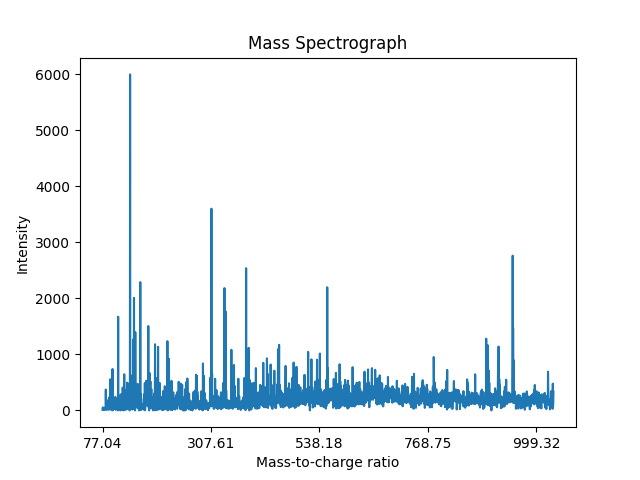
\includegraphics[width=0.6\linewidth]{assets/mass_spectrograph.png}
\caption{Mass Spectrograph: This is the artifact generated by Rapid Evaporative Ionization Mass Spectrometry (REIMS). The x-axis depicts the mass-to-charge ratio (m/z), and the y-axis depicts the relative abundance or intensity. The peaks on the chart represent the detection of ions. A taller peak indicates a greater abundance of ions with that particular mass-to-charge ratio detected by the instrument.}
\label{fig:mass-spectrograph}
\end{figure}

Compared to these traditional laboratory methods, REIMS offers significant advantages, especially with its ability to produce near-instantaneous results, making it ideal for in-situ (i.e., in the original place or on-site) applications \citep{Hendriks2025, Cai2025, Henderson2025}. As a 2024 review by \citet{Cafarella2024} highlights, its two primary application areas are clinical diagnostics and the agri-food sector. In clinical settings, it is used for real-time tissue classification in neurosurgery \citep{Hendriks2025}, differentiating degrees of fatty liver disease \citep{Eckel2025}, and evaluating venous leg ulcers in outpatient settings \citep{Pruekprasert2025}. Its use in the agri-food sector is a major, rapidly expanding field aimed at safeguarding food quality and security \citep{Cafarella2024, Henderson2025}. Recent food science applications include fish processing \citep{Black2017}, real-time pork breed and boar taint classification \citep{Gkarane2025, Verplanken2016}, and accurate lamb origin traceability \citep{Gao2025}. The versatility of REIMS is further shown by its use in entomology, where it can reliably determine the age and species of malaria-vector mosquitoes \citep{Wagner2025}. REIMS has consistently shown high accuracy in these various applications, with recent studies reporting accuracies of 80-94\% for medical diagnostics \citep{Pruekprasert2025, Wagner2025}, over 89-90\% for pork breed identification \citep{Gkarane2025}, 99.14\% for lamb origin traceability \citep{Gao2025}, and 100\% for in-vivo tumor identification \citep{Hendriks2025}. Other established applications include species of origin identification for meat products \citep{Balog2016}, fish species identification, and catch type identification \citep{Black2017}. Furthermore, it has detected adulteration with offal contamination in minced beef samples at concentrations as low as 1\% \citep{Black2019}.

A critical component of these applications, as highlighted in the 2024 review by \citet{Cafarella2024}, is the combination of REIMS data with chemometrics and machine learning to build classification models. The vast majority of current studies, in both clinical and food science, rely on traditional multivariate statistical methods. For example, high-accuracy classifications in glioblastoma, leg ulcer, and fatty liver analyses were achieved using Principal Component Analysis (PCA) and Linear Discriminant Analysis (LDA) \citep{Hendriks2025, Pruekprasert2025, Eckel2025}. Similarly, recent high-performance models for pork and lamb traceability were built using Orthogonal Partial Least Squares Discriminant Analysis (OPLS-DA), Support Vector Machines (SVM), and Random Forest \citep{Gkarane2025, Gao2025}. However, these traditional models are not always sufficient for modeling the highly complex, non-linear relationships within a full mass spectrum. This limitation is a key motivator for the work in this thesis. Recent 2025 research in food science has begun to demonstrate the superiority of deep learning; a study on coffee trait prediction found that Artificial Neural Networks (ANNs), a form of deep learning, significantly outperformed traditional PLS-DA by better capturing the complex relationships between the REIMS profiles and the modelled properties \citep{Cardoso2025}.

\section{Literature Review: The State of REIMS Data Analysis}
\label{sec:reims-lit-review}

The technique of REIMS analysis is relatively new, with existing literature on its data analysis methods falling into two main categories. The first group comprises foundational studies that introduced the REIMS technology and demonstrated its potential in medical applications, primarily for real-time tissue analysis using basic dimensionality reduction and linear classification. The second group builds on this foundation, applying REIMS to the field of food science, which led to the adoption of more advanced chemometrics and, very recently, foundational machine learning models. This section reviews these key works, analyzing their strengths and limitations to contextualize the contributions of this thesis.

\subsection{Foundational Studies: Establishing REIMS for In-Situ Tissue Analysis}

The initial development of REIMS focused on its application as a real-time analytical tool for biological tissue, particularly in medical settings. The pioneering work by \cite{Schaefer2009}
introduced REIMS as a novel technique for in vivo, in situ biomass analysis, demonstrating its ability to distinguish between malignant tumor cells and healthy tissue using Principal Component Analysis (PCA). This was advanced by
\cite{Balog2010}, who presented the first experimental setup for in vivo analysis in rats, achieving over 97\% accuracy in tissue identification using a PCA-Linear Discriminant Analysis (PCA-LDA) algorithm. The most high-profile application from this period was the development of the ``iKnife" by
\cite{Balog2013}, which used REIMS to analyze surgical smoke in real-time, matching histological diagnoses with 100\% accuracy and bringing significant publicity to the technique.

These foundational studies successfully established REIMS as a revolutionary technology capable of near-instantaneous analysis with no sample preparation. Their primary achievement was demonstrating extremely high accuracy and utility in a demanding real-world application like intraoperative diagnostics.

The analytical methods used in these early stages were limited to PCA and PCA-LDA. These techniques are primarily for dimensionality reduction and linear classification, and they are not well-suited for capturing the complex, non-linear patterns present in high-dimensional mass spectra. This reliance on simpler models represented a key area for future improvement.

\subsection{Advancements in Food Science: From Chemometrics to Machine Learning}

Building on the success in medical diagnostics, researchers began applying REIMS to address critical challenges in the food industry.
\cite{Balog2016} Demonstrated REIMS as a fast and effective method for meat product identification, achieving 100\% species identification accuracy and detecting adulteration at concentrations as low as 5\%. This application to food safety was further explored by
\cite{Verplanken2016}, who used an Orthogonal Partial Least Squares Discriminant Analysis (OPLS-DA) model to detect boar taint with over 99\% accuracy. The work of
Black et al. were particularly influential in this area. Their 2017 study \citep{Black2017} showed REIMS with OPLS-DA was a rapid, preparation-free alternative to genomic profiling for fish species identification, achieving 98.99\% accuracy. In 2019 \citep{Black2019}, they further demonstrated the technique's sensitivity by using it to detect offal adulteration in minced beef at concentrations as low as 1-5\%. This application of OPLS-DA for binary classification became a standard, with further studies successfully using it and similar multivariate techniques for identifying fish species like cod vs. oilfish \citep{Shen2020} and basa vs. sole \citep{Shen2022}.

This body of work successfully transitioned REIMS from a medical tool to a powerful instrument for food fraud and safety applications. The adoption of OPLS-DA represented a methodological step forward from PCA-LDA, providing a more sophisticated supervised learning approach for chemometric analysis.

However, while effective for specific tasks, the reliance on OPLS-DA and similar linear models was a limitation. Recognizing this, more recent research, as chronicled in reviews like \cite{Xue2025}, began to explore more advanced machine learning (ML) models to better capture non-linear patterns. This led to direct comparisons between traditional ML (e.g., Random Forest, SVM) and established chemometrics (e.g., PCA-LDA). A key study by \cite{De2023} on large-scale fish speciation found that while ML models were promising, traditional PCA-LDA could remain more robust and `industry-proof' on new test sets, highlighting an active debate in the field. Other work pairing ML with REIMS focused on new tasks and instrumentation. For example, \cite{Lu2024} successfully applied a K-Nearest Neighbors (KNN) model for the geographical authentication of fish, demonstrating a new application.

Most recently, this trend has progressed to deep learning, specifically Artificial Neural Networks (ANNs). In a study highly relevant to this thesis, \cite{Cardoso2025} demonstrated that ANNs outperformed traditional PLS-DA models for predicting coffee traits from LA-REIMS data. This work not only showed the superior predictive power of ANNs but also introduced novel methods for interpreting their model weights, beginning to address the `black-box' problem.

\subsection{Connecting to the Contributions of This Thesis}

The limitations and recent advancements of the existing literature directly motivate the core contributions of this thesis. While prior work established REIMS as a powerful data acquisition tool and recently began applying foundational ML and ANNs, it highlighted a clear need for state-of-the-art analytical methods to unlock its full potential. This thesis addresses these gaps in three key ways:

\begin{enumerate}
    \item Addressing the Analytical Gap: Where previous studies relied on traditional linear models (PCA-LDA, OPLS-DA) and, more recently, conventional ML (KNN, SVM) and foundational ANNs \citep{Cardoso2025}, this thesis introduces a suite of state-of-the-art deep learning architectures (e.g., Transformers, Mixture of Experts) capable of learning the complex, sequential, and non-linear patterns inherent in REIMS data.
    \item Addressing the Task Gap: This thesis moves beyond foundational classification (species identification, geographical origin) by formalizing and solving novel and more challenging problems, such as detecting graded levels of oil contamination and developing a completely new, self-supervised method for batch traceability (``SpectroSim").
    \item Enhancing Trust and Interpretability: While recent work has begun to develop methods for interpreting ANNs \citep{Cardoso2025}, this remains a significant challenge for more complex architectures. To overcome the black-box nature of these models, this thesis integrates advanced explainable AI (XAI) techniques (LIME and Grad-CAM), ensuring that model decisions are transparent and verifiable by domain experts, a crucial step for real-world adoption.
\end{enumerate}

\section{Advanced Deep Learning Architectures for REIMS Analysis}

The limitations of traditional statistical and foundational ML methods, as outlined in \Cref{sec:reims-lit-review}, have driven the exploration of sophisticated deep learning techniques to unlock the full potential of REIMS data. This section introduces the advanced architectures and strategies that form the core of this thesis's solution.

\subsection{Deep Learning}

\textbf{Deep learning} is a specialized subset of machine learning often based on artificial neural networks with multiple layers (i.e., deep architectures) to automatically learn hierarchical feature representations from raw data. The term deep refers to the depth of these layered networks, which can contain dozens or even hundreds of interconnected layers. Deep learning has been incredibly successful in handling complex, high-dimensional data across various domains \citep{Goodfellow2016}. The aforementioned capability to learn hierarchical feature representations from raw data makes them ideal for capturing the complex relationships found in REIMS mass spectra.

In order to appreciate it fully, here is a brief bibliographical history of deep learning, in chronological order. This is not an exhaustive list, but a representative sampling of some key papers that inform deep learning methodology and inspired the methods used in this thesis. In particular, those papers are:

\begin{itemize}
    \item \textbf{\cite{Linnainmaa1970}}
    Seppo Linnainmaa's Master's thesis was not initially about neural networks. However, it laid the mathematical foundation for the backpropagation algorithms. He proposed the reverse mode of automatic differentiation, a technique for efficiently calculating the gradient of a composite function by accumulating derivatives backwards from the output. This method proved most useful when you needed to compute the gradient of a function with a large number of input variables and a small number of output variables. Take, for example, a neural network, where the goal is to minimize a scalar loss function concerning millions of network weights. It would take over a decade for the application of neural networks to be found and popularized, Linnainmaa's work provided the foundational algorithm behind backpropagation for training deep, complex neural architectures.
    
    \item \textbf{\cite{Rumelhart1985}}
    This paper helped popularize the backpropagation algorithm for training Multi-layer Perceptrons (MLPs), or deep feedforward neural networks. While the core idea of backpropagation has already been discovered, this paper articulates the method and demonstrates its potential for learning complex internal representations in hidden layers. Rumelhart, Hinton, and Williams showed that error could be efficiently propagated backward through the network to adjust the weights. This paper is widely credited with starting the connectionist revival of the 1980s, and it lays the foundation for subsequent advances in deep learning. 
    
    \item \textbf{\cite{LeCun1989b}}
    Yann LeCun and his colleagues at Bell Labs provided one of the earliest and most convincing applications of backpropagation, particularly when combined with their Convolutional Neural Networks (CNNs). Their application of backpropagation to CNNs was for recognizing handwritten zip codes for the U.S. Postal Service. It demonstrates the ability of these networks to learn hierarchical features directly from raw pixel data, performing automatic feature extraction, it achieving high accuracy and robustness. They create a system that could outperform traditional pattern recognition techniques by integrating concepts like local receptive fields, shared weights, and backpropagation for training. The success of both validated backpropagation for real-world tasks, and also demonstrated the efficacy of the CNN architecture. 
    
    \item \textbf{\cite{Bromley1993}}
    Jane Bromley, Yann LeCun, and his colleagues developed Siamese networks for pair-wise comparison tasks. Siamese networks were first developed for signature verification, a task that involves comparing a known authentic signature with a query signature to determine if they were written by the same person. The goal was to predict whether a signature was genuine or forged. Siamese networks achieve this by using two identical neural networks that share the same weights and architecture. One network processes a reference input (e.g., an authentic signature or a known sample), while the other processes the query input (e.g., the signature being tested or an unknown sample). The outputs from both networks are then combined using a distance metric to produce a similarity score. For instance, the original paper used Euclidean distance; a smaller distance indicated higher similarity, suggesting the query was genuine or from the same source, while a larger distance suggested it was forged or from a different source.
    
    \item \textbf{\cite{Hochreiter1997}}
    Sepp Hochreiter and Jürgen Schmidhuber introduced the Long Short-Term Memory (LSTM) architecture. The LSTM addresses the vanishing gradient problem that plagued simple Recurrent Neural Networks (RNNs) and produced unstable training dynamics for tasks involving long-term dependencies. LSTMs integrate specialized memory cells and gating mechanisms (i.e., input, output, and forget gates) that allow the network to selectively remember or forget information over time. This design enables LSTMs to have long-term memory, allowing them to capture and exploit context from distant past inputs. This made them exceptional for a wide variety of sequence modelling tasks, e.g., speech recognition, machine translation, and time series analysis, where they were a dominant approach for many years. 
    
    \item \textbf{\cite{LeCun1998}}
    Yann LeCun, Léon Bottou, Yoshua Bengio, and Patrick Haffner designed the LeNet-5 architecture, a Convolutional Neural Network (CNN) that was highly optimized for document recognition tasks, i.e., handwritten digit and character recognition. LeNet-5 integrated convolutions with learnable filters, subsampling (i.e., pooling) layers for spatial invariance, and fully connected layers, all trained with end-to-end gradient-based learning. The paper highlighted the importance of automatic feature extraction. LeNet-5 is a foundational model that influenced later architectures and breakthroughs in computer vision. 
    
    \item \textbf{\cite{Krizhevsky2012}}
    Alex Krizhevsky, Ilya Sutskever, and Geoffrey Hinton developed ``AlexNet,'' a deep convolutional neural network that won the ImageNet Large Scale Visual Recognition Challenge (ILSVRC) 2012, beating the other traditional computer vision models of the time. AlexNet's success was attributed to its deep architecture, the use of Rectified Linear Units (ReLUs) activation function, dropout for regularization, and efficient GPU training. This watershed moment convinced the computer vision community of the power of deep learning. This paper, the advent of big data, and GPU training, together unfroze the AI winter and ignited the modern deep learning revolution. 
    
    \item \textbf{\cite{Kingma2013}}
    Diederik Kingma and Max Welling introduced Variational Autoencoders (VAEs), providing an influential framework for deep generative modelling by combining concepts from variational Bayesian methods and neural networks. VAEs learn a probability distribution of the input data, allowing them to generate synthetic data samples that were not present in the training set. VAES learn a probabilistic encoder that maps input data to a distribution in the latent space (e.g., typically Gaussian), and a probabilistic decoder that maps points from the latent space back to the data space, i.e., the decoder reconstructs the data from the latent representation. 
    
    \item \textbf{\cite{Goodfellow2014}}
    Ian Goodfellow and his collaborators introduced Generative Adversarial Networks (GANs) as a new framework for generative AI. A GAN has two neural networks, a generator and a discriminator, trained simultaneously in a min-max game to reach a Nash equilibrium: the generator learns to produce data that matches the training set, and the discriminator learns to distinguish the training set from the synthetic data. This adversarial process leads to the generator producing more realistic samples over time. GANs quickly became one of the most popular ideas in deep learning. It leads to rapid progress in generating high-fidelity images, videos, and more. GANs inspired a vast amount of research in generative AI and unsupervised learning. 
    
    \item \textbf{\cite{Kingma2014}}
    Diederik P. Kingma and Jimmy Ba introduced Adaptive Moment Estimation (Adam), a highly popular and effective optimization algorithm used in deep learning. Adam computes adaptive learning rates for each parameter. By integrating estimates of both the first moment (i.e., mean) and the second moment (i.e., uncentered variance) of the gradients, Adam combines the key ideas of Momentum and RMSprop, two other popular optimization algorithms. It is computationally efficient, requires little memory, and is well-suited for large-scale machine-learning problems with many parameters. Due to strong empirical performance and ease of use, Adam quickly became the most popular and often default optimization algorithm for training deep learning models. 
    
    \item \textbf{\cite{Srivastava2014}}
    Srivastava, Hinton, Krizhevsky, Sutskever, and Salakhutdinov introduced Dropout, a regularization technique to combat overfitting in large neural networks. Enabled only during training, Dropout randomly turns off a subnetwork of neurons for each training batch, preventing neurons from co-adapting too much and encouraging them to learn more robust features. Conceptually, it efficiently approximates a bagged ensemble of sub-neural networks. Dropout significantly improved the generalization performance in most cases and has now become an indispensable tool for deep learning practitioners. 
    
    \item \textbf{\cite{He2016}}
    Kaiming He and his colleagues introduced Deep Residual Networks (ResNets) to address the problem of degradation in very deep networks (where deeper models performed worse). ResNet, an extension of Convolutional Neural Networks (CNNs), employs skip connections or shortcuts between layers. This creates gradient superhighways that allow gradients to propagate more easily through extremely deep architectures. This made it feasible to train neural networks with hundreds of layers. On computer vision benchmarks like ImageNet, ResNet achieved record-breaking results, demonstrating that, when managed correctly, network depth is crucial for improving model performance. This has influenced future network designs profoundly. 
    
    \item \textbf{\cite{Vaswani2017}}
    Vaswani and his colleagues introduced the Transformer architecture, which revolutionized sequence modeling. Departing from traditional deep learning architectures such as convolutional and recurrent layers for sequence-to-sequence tasks, the Transformer uses attention mechanisms, specifically self-attention, to draw global dependencies between input and output. Its ability for parallelism allows for training on much larger datasets when compared to RNNs. Some more key innovations for the transformer were multi-head attention and positional encodings. The Transformer's effectiveness, efficiency, and scalability quickly made it the default architecture for NLP tasks, and this architecture has also been successfully applied to many other domains. 
    
    \item \textbf{\cite{Devlin2018}}
    Jacob Devlin and his colleague introduced Bidirectional Encoder Representations from Transformers (BERT), building upon Transformers and pre-training. BERT was designed to pretrain deep bidirectional representations by joint conditioning on both left and right context in all layers, using novel pre-training tasks, such as Masked Language Modeling (MLM) and Next Sentence Prediction (NSP). Once pretrained on a large text corpus, BERT could be fine-tuned with just one additional output layer to create state-of-the-art models for a wide range of NMLP tasks without substantial task-specific architecture changes. This ushered in the era of large-scale pretrained language models. 
    
    \item \textbf{\cite{Brown2020}}
    Brown and his colleagues unveiled Generative Pre-Trained Transformer 3 (GPT-3). A large language model with 175 billion parameters, proving the extreme scaling capabilities of the Transformer architecture. The authors demonstrated that a dramatic increase in model size, dataset, and computation could achieve remarkable performance on many NLP tasks without any fine-tuning, with GPT-3 matching or exceeding state-of-the-art fine-tuned models. The so-called emergent capabilities of large language models (LLMs), such as few-shot or in-context learning (i.e., where models could perform a new task without retraining by being provided a natural language description and a few examples as an input prompt), have inspired a new wave of deep learning research into the scaling of LLMs. The scaling laws of LLMs are demonstrated in \Cref{fig:parameters-comparison}.
    
    
    \begin{figure}
    \centering
    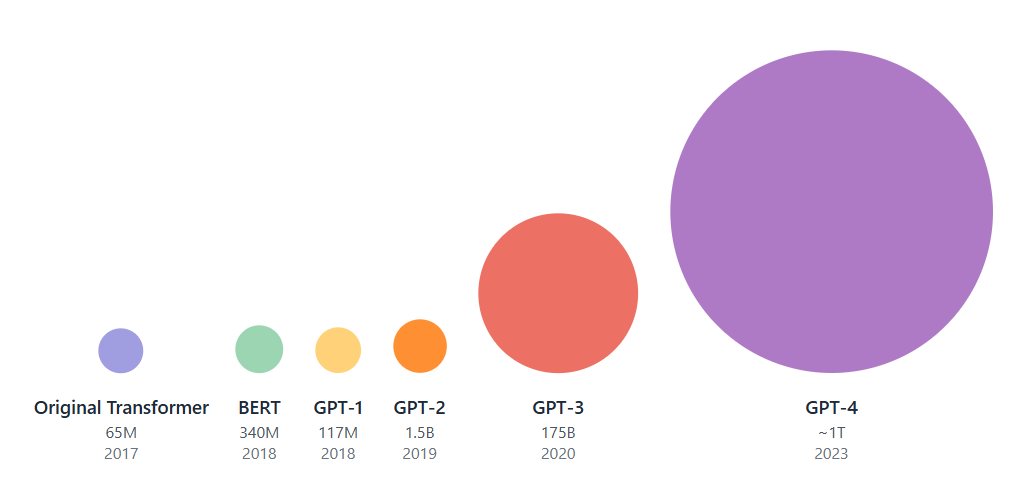
\includegraphics[width=\linewidth]{assets/parameters-comparison.png}
    \caption{Illustrated here is a comparison of Transformer models, with each circle's size representing its approximate number of parameters. This visualization highlights the prominent scaling laws observed in large language models, particularly the exponential increase in parameters across successive iterations of the GPT series (GPT-1, GPT-2, GPT-3, GPT-4). For context, the original Transformer and BERT models are also included.}
    \label{fig:parameters-comparison}
    \end{figure}
    
    \item \textbf{\cite{Ho2020}}
    Jonathan Ho and his collaborators introduced Denoising Diffusion Probabilistic Models (DDPMs), a new class of generative AI models based on diffusion. These diffusion models achieved state-of-the-art results in image synthesis, dethroning GANs from their previous perch. Diffusion models work by systematically destroying an image through a forward diffusion process (i.e., gradually adding noise) and then learning a reverse diffusion process that restores the image. This new approach, with a specific training objective and sampling procedure, demonstrated high efficacy for generating high-fidelity images. DDPM's success led to a large interest in diffusion models within the deep learning community. Now, many state-of-the-art image, audio, and video generation systems consist of diffusion models.
    
    \item \textbf{\cite{Gu2023}}
    Albert Gu and Tri Dao introduced Mamba, a type of State Space Model (SSM) that incorporates a selection mechanism inspired by gating in RNNs and the efficiency of convolutional approaches. It serves as an efficient alternative to Transformer-based architectures, especially for very long sequences. Its key contribution is the capability to model long-range dependencies with linear time complexity with regard to sequence length, a large improvement over the quadratic complexity of standard Transformers. This is achieved through a hardware-aware design that leverages parallel scans for efficient computation during training and inference. 
    
    \item \textbf{\cite{Liu2024}}
    Inspired by the Kolmogorov-Arnold representation theorem, Ziming Liu, Max Tegmark, and colleagues recently introduced Kolmogorov-Arnold Networks (KANs). This novel neural network architecture distinguishes itself by placing learnable activation functions (modeled as splines) on its edges, while nodes perform simple summations. A key advantage of KANs is their enhanced interpretability, allowing a direct mathematical expression of the network to be derived, thereby mitigating the black-box nature of traditional neural networks. Their design also grants them high efficiency in approximating complex functions.
\end{itemize}

\subsection{Stacking Ensembles}

Ensemble theory, through the lens of Wolpert's Stacked Generalization \citep{Wolpert1992}, is a framework for improving the predictive accuracy of machine learning by combining multiple models. The central goal is to create a more powerful and robust classifier than any single model could achieve on its own by leveraging the wisdom of the crowds. This approach is particularly effective when the individual models are independent, complementary, and diverse.

The architecture proposed by Wolpert consists of two levels. The first level contains multiple independent base models, referred to as level-0 generalizers. The predictions from these base models are then used as input features for a single, higher-level level-1 generalizer, or meta-model. In a stacked voting ensemble, this meta-model is often implemented as a learnable weighted combination of the predictions from the level-0 models.

The objective of this framework is for the meta-model to learn how to optimally combine the outputs from the base models. By training the weights of the voting classifier, the ensemble learns to correct for the individual errors and biases of each base model. This intelligent combination of diverse models, each with its own strengths and weaknesses, ultimately reduces the overall generalization error and leads to a more robust final prediction. This principle is most effective when the errors of the base models are not perfectly correlated, as their individual idiosyncrasies can then cancel each other out during the aggregation process.

\subsection{Transformers}

\textbf{Transformers} \citep{Vaswani2017} have gained significant prominence among deep learning architectures. Initially, they were only applied to the field of Natural Language Processing (NLP) \citep{Ansar2024,Fields2024}, but now they have been applied to a variety of domains \citep{LaiDang2024,Li2021,Lee2024}. Some key contributions of the Transformer are the self-attention mechanism and multi-head attention (note: positional embeddings are excluded as we opt for No Positional Embeddings (NoPE) \citep{Wang2024} in the transformer models presented in this thesis).

\subsubsection{Self-Attention}

An \textbf{attention} function transforms a query vector and a collection of key-value vector pairs into an output vector. This output is calculated as a weighted sum of the value vectors, with the weight for each value derived from a compatibility measure between the query and its associated key.

\begin{figure}
\centering
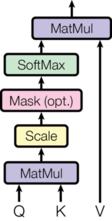
\includegraphics[width=0.15\linewidth]{assets/scaled-dot-product.png}
\caption{
This figure illustrates the Scaled Dot-Product Attention mechanism \citep{Rush2018}, a core component of self-attention. It takes queries ($Q$) and keys ($K$) of dimension $d_k$, and values ($V$) of dimension $d_v$. Attention weights are computed by taking the dot product of $Q$ with all $\mathbf{K}$s, scaling by $\sqrt{d_k}$, and applying a softmax function. These weights are then applied to the $\mathbf{V}$s to produce the output.}
\label{fig:self-attention}
\end{figure}

For each input element, three learned linear transformations are applied to generate:
\begin{itemize}
\item \textbf{Query (\texttt{Q})}: What an element is looking for.
\item \textbf{Key (\texttt{K})}: What an element offers.
\item \textbf{Value (\texttt{V})}: The actual information to be aggregated.
\end{itemize}

Given a query, key, and value, we compute the Scaled Dot Product Attention as follows:

\[ \texttt{Attention} (Q,K,V) = \texttt{softmax} (\frac{QK^{\top}}{\sqrt{d_k}}) V \]

\textbf{Self-attention} operates within a single sequence. It allows each element of the sequence to learn its relationship and importance to all the other elements within the same sequence. In self-attention, the query, key, and value vectors are all derived from the same sequence. Unlike Recurrent Neural Networks (RNNs) \citep{Rumelhart1985} that process sequentially, self-attention can be done in parallel. Therefore, it can efficiently model long-range dependencies and contextual relationships regardless of their distance.

\subsubsection{Multi-head Attention}

\textbf{Multi-Head Attention} is an extension of the self-attention mechanism, designed to enhance the model's ability to focus on different parts of the input sequence from various perspectives or representation subspaces.

\begin{figure}
\centering
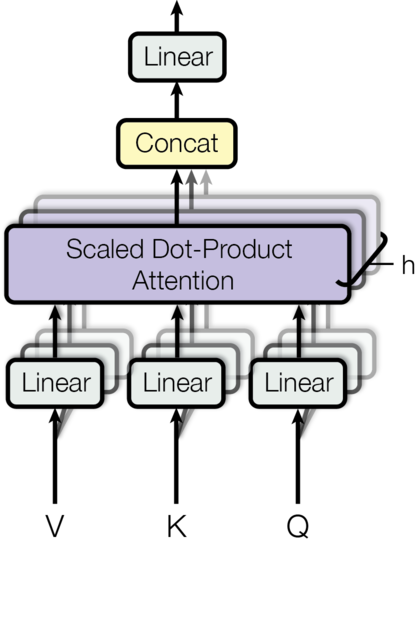
\includegraphics[width=0.3\linewidth]{assets/multi-head-attention.png}
\caption{Multi-head attention \citep{Rush2018} enhances a model's ability to capture complex relationships by allowing it to jointly focus on distinct representation subspaces at different positions. A single attention head's averaging effect would otherwise obscure such nuanced information.}
\label{fig:multi-head-attention}
\end{figure}

While single self-attention may restrict a model to learning only one type of relationship, Multi-Head Attention addresses this by performing the attention mechanism multiple times in parallel, each with its own independent set of learned linear projections. This allows the model to jointly attend to information from diverse representation subspaces at different positions, thereby learning richer and more varied relational patterns.

Specifically, for $H$ heads, the input Query ($Q$), Key ($K$), and Value ($V$) matrices are first linearly projected into distinct lower-dimensional subspaces for each head. The standard scaled dot-product attention is then applied independently to these projected $Q_h$,$K_h$, and $V_h$ sets. Finally, the outputs from all H heads are concatenated and linearly transformed back to the original model dimension, allowing the model to collectively leverage diverse contextual information. This process is illustrated in \Cref{fig:multi-head-attention}.

\subsection{Mixture of Experts (MoE)}

The \textbf{Mixture of Experts (MoE)} architecture is a neural network design that combines multiple specialized subnetworks, known as experts, coordinated by a trainable gating network \citep{Jacobs1991}. The gating network dynamically routes input data (or parts of it) to the expert(s) deemed most suitable for processing that specific information. This selective activation allows MoE models to scale to a very large number of parameters without a proportional increase in computational cost per inference, as only relevant experts are activated for any given input. When integrated into Transformer architectures (MoE Transformers) \citep{Kaiser2017,Guo2025,Jaech2024}, typically by replacing standard feed-forward network layers with MoE layers, this approach can enhance model capacity and adaptability, allowing the model to develop specialized representations for different aspects of the data or tasks \citep{Kaiser2017}. This makes MoE Transformers particularly promising for handling diverse and complex datasets like those generated by REIMS across various fraud detection tasks.

\subsection{Pretrained Transformers}

\textbf{Unsupervised pretraining} is a powerful technique where a Transformer is pretrained to learn general-purpose embeddings from data that doesn't explicitly require labels (i.e., unsupervised) before being fine-tuned on a specific downstream task. This technique allows the Transformer to capture the underlying structure of the data, which is helpful when training data is scarce. Two prominent approaches to pre-training are demonstrated by GPT \citep{Radford2018} and BERT \citep{Devlin2018}. The Generative Pretrained Transformer (GPT) (\citep{Radford2018}) was trained to predict the next word in sequence, learning a left-to-right unidirectional representation. Alternatively, BERT \citep{Devlin2018} introduced Masked Language Modelling (MLM) as a pretraining task. In MLM, some tokens in the input sequence are randomly masked, and the model is trained to predict the masked tokens using the context. This forces the model to learn deep bidirectional relationships within the data, creating robust embeddings to transfer to downstream tasks.

\subsection{Transfer Learning}

\textbf{Transfer learning} \citep{Bozinovski1976,Tan2018} is a machine learning paradigm where knowledge gained from solving one problem (the source task) is applied to a different but related problem (the target task). In practice, a model is often pre-trained on a large dataset for a general task and then its learned parameters and feature representations are transferred to initialize a new model for a target task, which is then fine-tuned on a smaller, task-specific dataset. This technique can significantly reduce the amount of labeled data needed for the target task, shorten training times, and often improve performance, especially when the source and target domains share underlying patterns. However, the effectiveness of transfer learning can be asymmetric and task-dependent. While it can yield significant improvements in some cases, it may offer little benefit or even degrade performance in others. Understanding these dynamics is crucial for their effective application.

\subsection{Contrastive Learning}

\textbf{Contrastive learning} is a machine learning technique that learns effective representations by contrasting positive and negative pairs of data instances—distinct from class labels—mapping similar instances closer in the embedding space and dissimilar ones further apart. It excels in supervised and self-supervised settings, notably in computer vision \citep{Bromley1993,Jing2022} and natural language processing \citep{Zhu2022}. In supervised contrastive learning, labeled data are used to train models to distinguish similar from dissimilar instances, while in self-supervised learning, models are trained using unlabeled data, forming pairs via augmentation to capture specific features like edges or semantic similarities, enhancing performance over traditional methods in tasks like classification.

SimCLR \citep{Chen2020a}, exemplifies self-supervised contrastive learning, using a backbone like ResNet \citep{He2016} to process augmented views of the same input. It applies NT-Xent loss to align representations of these views (positive pairs) while separating different inputs (negative pairs), identifying positive pairs as augmented versions of the same data point without needing labels. This enables pre-training on large unlabeled datasets for downstream tasks like image classification and object detection, leveraging augmentation for effective representation learning.

However, SimCLR faces several limitations. It demands high computational resources, necessitating large batch sizes and extensive training for optimal performance \citep{Chen2020b}. The method's effectiveness is heavily dependent on data augmentations, as poor choices—like random cropping—can significantly impair the quality of learned representations \citep{Chen2020a}. Furthermore, SimCLR struggles with small datasets, often requiring specific tweaks to be effective in limited data regimes \citep{Kinakh2021}. Finally, without robust augmentation, SimCLR can lose its self-supervised nature, inadvertently relying on labeled data for effective representation learning \citep{Chen2020a}.

\section{Explainable AI for Model Trust and Interpretability}

A significant challenge in deploying advanced deep learning models, as noted in recent REIMS literature \citep{Cardoso2025}, is their ``black-box" nature. To address this and build trust for real-world adoption, this thesis integrates Explainable AI (XAI) techniques.

\cite{Ribeiro2016} introduced \textbf{Local Interpretable Model-agnostic Explanations (LIME)}, a post-hoc explainable AI technique that can explain the predictions of any black-box model, particularly applicable to those from deep learning. LIME approximates a complex model with a simpler interpretable one (for example, a linear regression model) in the local area of a specific instance. LIME creates many perturbed versions of an input instance to see how the predictions change. Through this process, it identifies the important features that influence the model's decisions for that instance. This thesis uses LIME explanations to explore the black-box Transformer models and their variants proposed.

\cite{Selvaraju2017} proposed \textbf{Gradient-weighted Class Activation Mapping (Grad-CAM)}, another technique for producing visual explanations of the decision process behind deep learning models. Grad-CAM works by using the gradients of the target class that flow through the final feature extraction layer of the model during backpropagation. This process generates an ``average correct Grad-CAM," which highlights important features that consistently contribute to accurate classification. This thesis implements a 1-dimensional Grad-CAM for Transformers that utilizes the gradients of the final attention layer to identify the important features behind correct classifications.

\section{Summary}

The challenge of food safety in fish processing requires a move beyond traditional analytical methods. The literature shows a clear progression: from foundational PCA/PCA-LDA and OPLS-DA to more recent explorations of conventional ML and foundational ANNs. While REIMS provides a powerful tool for rapid data acquisition, its true potential can only be realized by coupling it with advanced machine learning techniques that can model the complex, high-dimensional, and sequential nature of its data. This thesis directly addresses this gap. It proposes state-of-the-art deep learning architectures, particularly Transformers and their MoE variants, to solve novel, complex tasks like graded contamination and self-supervised batch traceability. Furthermore, by integrating XAI, it addresses the critical need for model interpretability, paving the way for robust, automated, and trustworthy systems for quality assurance in fish processing.